\subsection{Документирование плагинов}

На данный момент основной репозиторий находится на ресурсе GitHub. Данный ресурс использует язык разметки MarkDown (подробнее в разделе~\ref{sec:markdown}) и автоматически добавляет файл <<Readme.md>> к описанию плагина, если этот файл присутствует. В связи с этим было решено создать документацию плагинов, используя MarkDown. Документация должна включать в себя:

\begin{enumerate}
  \item Название плагина;
  \item Версию плагина;
  \item Автора плагина;
  \item Описание плагина;
  \item Требуемую операционную систему;
  \item Версию ПО, с которым этот плагин работает;
  \item Основные методы плагина с описанием входов и выходов.
\end{enumerate}

Результат разработанной документации можно наблюдать на странице плагина в репозитории (рис.~\ref{bok_1:bok_1}).

\begin{figure}[h!]
\center{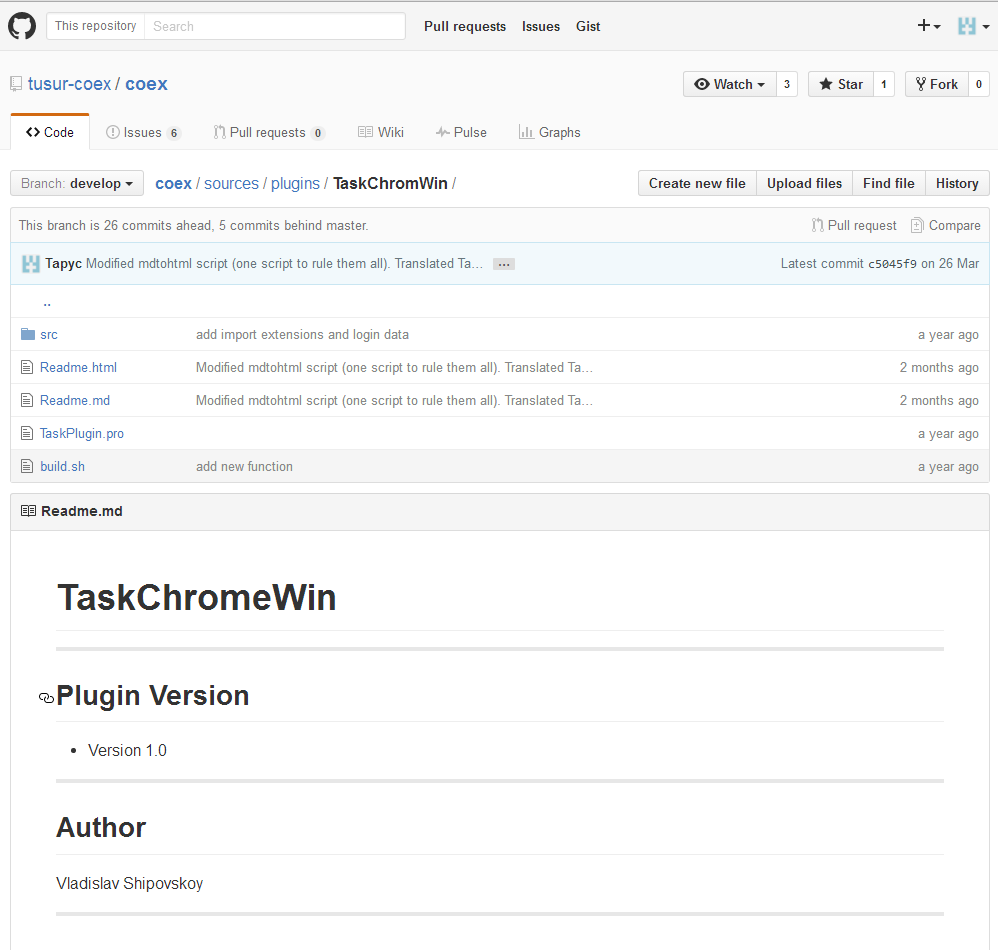
\includegraphics[width=0.8\linewidth]{bok_1}}
\caption{ Документация в веб-интерфейсе репозитория }
\label{bok_1:bok_1}
\end{figure}

Поскольку проект <<COEX>> имеет свою собственную веб-страницу, данную документацию также необходимо преобразовать в формат HTML, чтобы затем добавить на веб-страницу проекта. Для преобразования был разработан небольшой скрипт на языке Python (приложение ~\ref{apx:mdtohtml}). На рисунке ~\ref{bok_2:bok_2} можно наблюдать ту же документацию, но в формате HTML.

\begin{figure}[h!]
\center{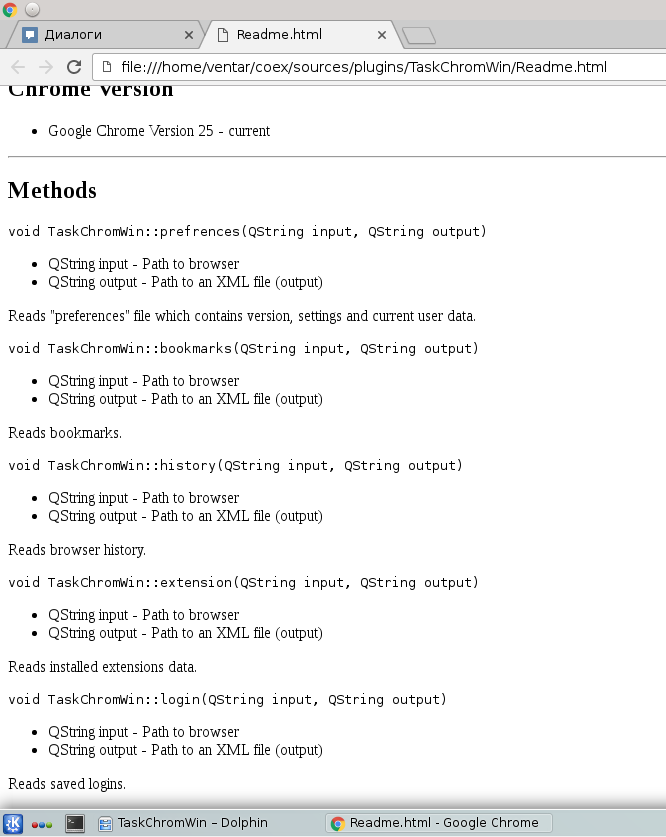
\includegraphics[width=0.9\linewidth]{bok_2}}
\caption{ Документация в формате HTML }
\label{bok_2:bok_2}
\end{figure}

\clearpage
\subsection{Разработка и внедрение копии жесткого диска}

Поскольку большое количество плагинов <<COEX>> обращается к жесткому диску для поиска тех или иных файлов, что в свою очередь создает серьезную нагрузку на него, то было решено модифицировать архитектуру проекта с целью хранения копии информации о жестком диске. Данную информацию решено было хранить как поле объекта <<config>>, к которому будут обращаться остальные плагины. Поле представляет из себя класс <<Hdd>> с атрибутом типа QList<QDir> (приложение ~\ref{apx:hddclass}). Данный тип был выбран, поскольку он позволяет хранить данные о всех директориях и файлах внутри них, а также предоставляет удобные интерфейсы для доступа к ним. Методы класса <<Hdd>>:

\begin{enumerate}
  \item Hdd::Hdd(QString path);
  \item Hdd::~Hdd();
  \item QFileInfoList getFiles(QStringList wildcardlist);
  \item QFileInfoList getFiles(QString wildcard).
\end{enumerate}

Метод <<Hdd::Hdd(QString path)>> является конструктором класса. Переменная <<path>>, подаваемая на вход метода является путем до начальной папки. Конструктор с помощью экземпляра класса <<QDirIterator>> посещает каждую папку в начальной папке и сохраняет данные о ней в переменную типа <<QDir>>, после чего добавляет эту переменную к массиву <<QList<QDir>>>, и наконец сохраняет полученный массив как поле класса. Алгоритм конструктора можно увидеть на рисунках~\ref{bok_6:bok_6} и~\ref{bok_7:bok_7}.

\begin{figure}[h!]
\center{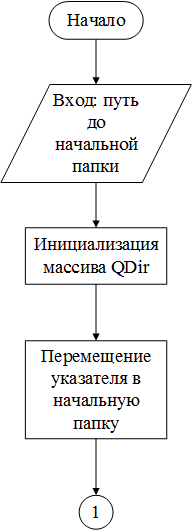
\includegraphics[width=0.3\linewidth]{bok_6}}
\caption{ Алгоритм конструктора класса <<Hdd>> }
\label{bok_6:bok_6}
\end{figure}

\begin{figure}[h!]
\center{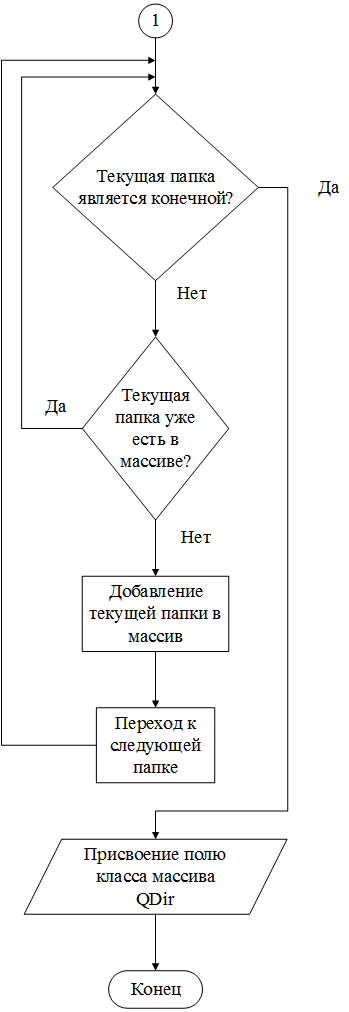
\includegraphics[width=0.5\linewidth]{bok_7}}
\caption{ Продолжение алгоритма конструктора класса <<Hdd>> }
\label{bok_7:bok_7}
\end{figure}

Метод <<Hdd::~Hdd()>> является деструктором класса.

Метод <<QFileInfoList getFiles(QStringList wildcardlist)>> возвращает объект <<QFileInfoList>> для всех файлов, которые соответствуют заданному массиву масок <<wildcardlist>>. Алгоритм метода можно увидеть на рисунке ~\ref{bok_9:bok_9}.

\begin{figure}[h!]
\center{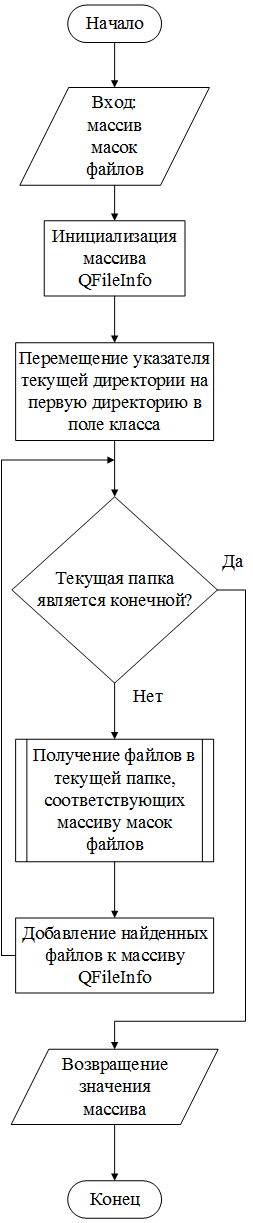
\includegraphics[width=0.3\linewidth]{bok_9}}
\caption{ Алгоритм метода <<getFiles>> класса <<Hdd>> }
\label{bok_9:bok_9}
\end{figure}

Метод <<QFileInfoList getFiles(QString wildcard)>> выполняет ту же функцию, что и прошлый метод. Он является перегрузкой прошлого метода и принимает на вход одну маску вместо массива. Алгоритм метода можно увидеть на рисунке ~\ref{bok_8:bok_8}.

\begin{figure}[h!]
\center{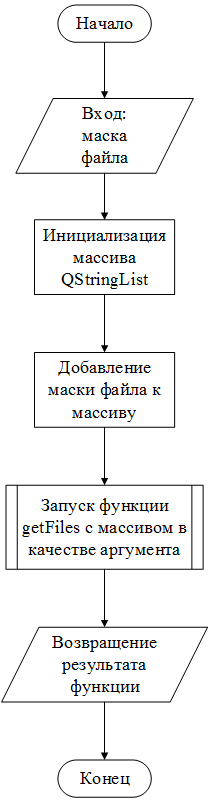
\includegraphics[width=0.3\linewidth]{bok_8}}
\caption{ Алгоритм перегруженного метода <<getFiles>> класса <<Hdd>> }
\label{bok_8:bok_8}
\end{figure}

После разработки архитектуры класса, он был внедрен в <<скелет>> проекта. Класс конструируется перед работой плагинов, но после определения операционной системы.

\begin{figure}[h!]
\center{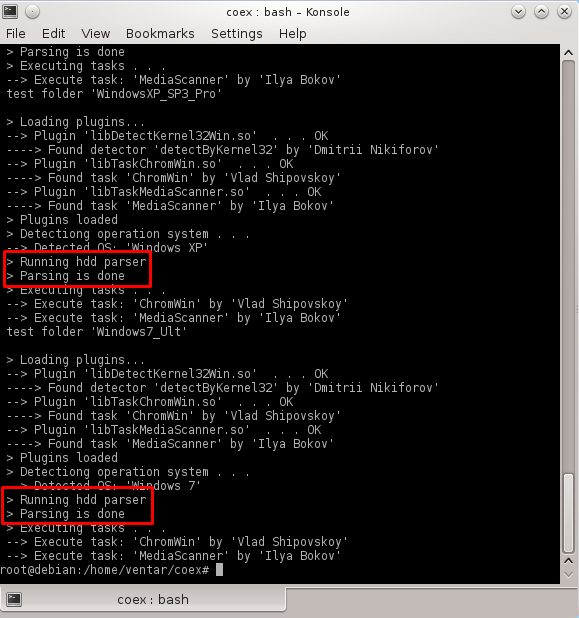
\includegraphics[width=1\linewidth]{bok_3}}
\caption{ Работа класса <<Hdd>> при запуске <<COEX>> }
\label{bok_3:bok_3}
\end{figure}

Далее необходимо было изменить плагины, таким образом, чтобы они обращались к сохраненной копии диска вместо самого диска. Таким образом были изменены два плагина - <<TaskMediaScanner>> и <<TaskChromeWin>>.

Теперь перед нами стояла задача сравнить нагрузку диска до и после внедрения класса <<Hdd>>. Поскольку нами использовался удаленный репозиторий и система контроля версий git, то это не составило проблемы по причине того, что разработка класса велась в отдельной <<ветке>>.

Было решено с помощью утилиты iotop замерить использование жесткого диска (в КБ/с) несколько раз до и после введения нового плагина и отфильтровать полученные результаты, чтобы учитывать исключительно нагрузку, создаваемую программой <<COEX>>. Для этого был разработан мультипоточный скрипт на языке Python, запускающий отдельно утилиту <<iotop>> и <<COEX>> и фильтрующий результаты, сохраняемые утилитой <<iotop>> (приложение ~\ref{apx:diskusage}):

\begin{figure}[h!]
\center{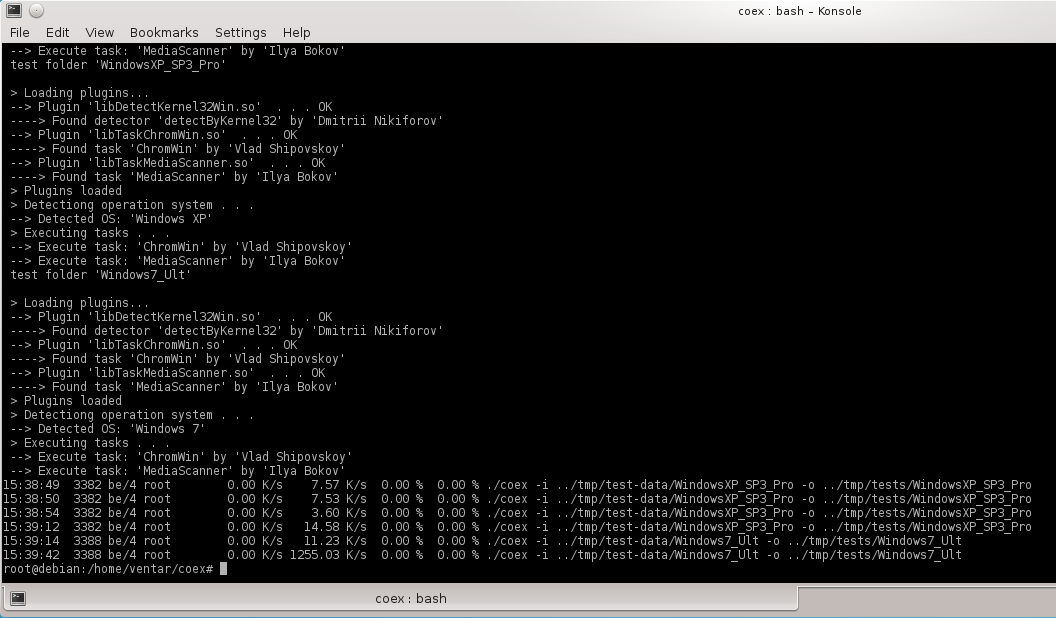
\includegraphics[width=1\linewidth]{bok_4}}
\caption{ Результат работы скрипта }
\label{bok_4:bok_4}
\end{figure}

Далее результаты были обработаны, и на основании их был построен график, показывающий нагрузку на жесткий диск до и после внедрения класса <<Hdd>>. Было решено оставить по 10 итераций на каждое измерение, поскольку после этого количества разница между итерациями была минимальна и уже прослеживалась значимая разница между измерениями.

\begin{figure}[h!]
\center{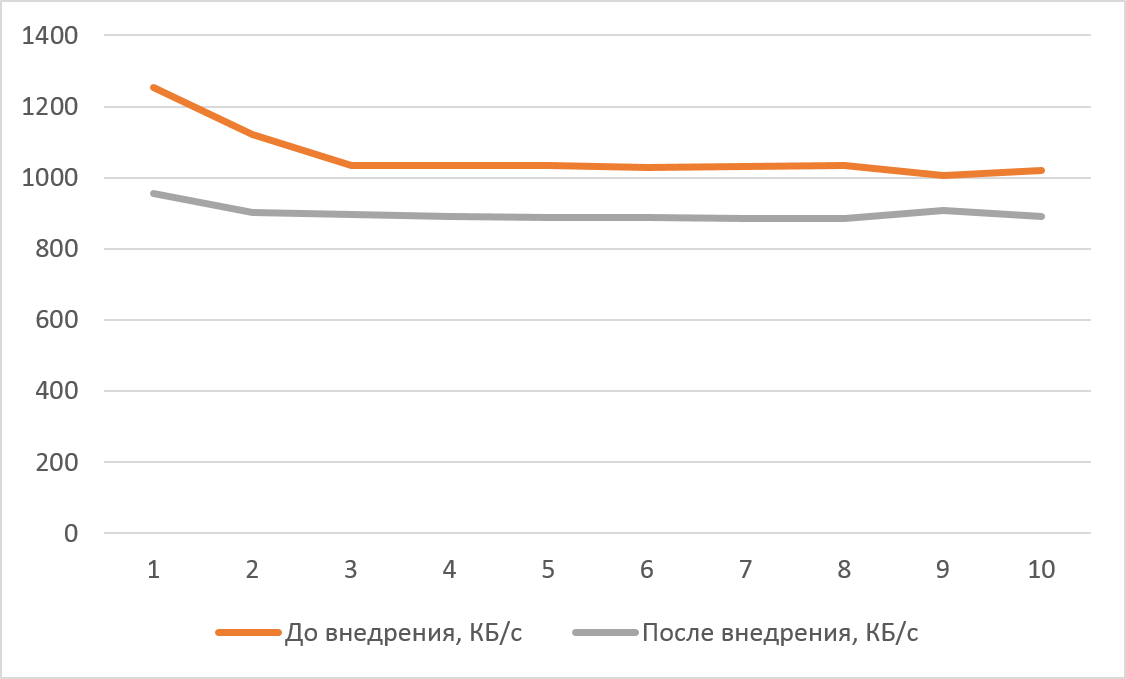
\includegraphics[width=1\linewidth]{bok_5}}
\caption{ Сравнение нагрузки на жесткий диск до и после изменения архитектуры }
\label{bok_5:bok_5}
\end{figure}

Из графика видно, что даже при изменении всего двух плагинов для использования новой архитектуры нагрузка на диск заметно снизилась. Так как на данный момент в проекте <<COEX>> имеется 17 рабочих плагинов, преобразование каждого из них должно сильно сказаться на нагрузке жесткого диска в лучшую сторону.

\clearpage
